
\chapter{Механизм поддержания продольных вихрей}



\section{Бегущая волна}

Как было показано в предыдущем разделе, в основе механизма самоподдержания решения на сепаратрисе лежит бегущая вниз по порыву волна. Оказывается возможным получить аналогичную волну в более простой форме. Длину волны, возникающей в модельном порыве, можно оценить в $5R$. Если применить метод поиска решения на сепаратрисе к расчетной области длиной $L_x = 5R$, то решение на сепаратрисе выходит на режим бегущей волны, двигающейся в низ по течению. В подвижной системе отсчета решение оказывается стационарным, что делает его еще более доступным для исследования, чем модельный порыв. Исследование этой бегущей волны показало, что она качественно воспроизводит многие особенности модельного порыва, а также позволило установить новые детали механизма самоподдержания, связанные с образование продольных вихрей. Применимость полученных при исследовании бегущей волны результатов к модельному порыву позже будет продемонстрированная отдельно. 


Бегущая волна была найдена также при $\Re = 2200$, скорость её сноса оказалась равна $c_f = $

Как и при исследовании модельного порыва, разделим поле скорости бегущей волны на стационарную и пульсационную составляющею. Осреднеие по времени в случаемоедльного порыва проводилось в системе отсчета, связанной с порывом, в которой бегущая волна, бегущая вниз по порыву волна оказывалась подвижной. 


\section{Механизм образования продольных вихрей.}

Продольные вихри в стационарной составляющей движения возникают в результате нелинейного взаимодействия пульсаций. Это, в частности, подтверждается фактом совпадения областей концентрации продольных вихрей и пульсаций вдоль трубы. Прояснить процесс формирования продольных вихрей позволяет анализ уравнения, описывающего эволюцию продольной завихренности, полученного применением оператора Ротора к уравнению Навье-Стокса \eqref{NSeq_cf}:
\begin{equation}\label{ox_eq}
\pd{\omega_x}{t} - \nu\nabla^2 \omega_x =  -  (\v - \c_f, \nabla) \omega_x + (\om, \nabla) v_x
\end{equation}
Здесь $\om = (\omega_x, \omega_r, \omega_\theta) = \rot \v$ --- вектор завихренности, $\c_f$ --- скорость перемещения системы отсчета. Уравнение для стационарной составляющей продольной завихренности получается после осреднения \eqref{ox_eq} по времени в системе отсчета, связанной с порывом:
\begin{equation}\label{OX_eq}
\pd{\Omega_x}{t} - \nu\nabla^2 \Omega_x = - (\V - \c_f, \nabla) \Omega_x + (\Om, \nabla) V_x - \overline{(\v', \nabla) \omega'_x}^t + \overline{ (\om', \nabla) v'_x }^t
\end{equation}
Здесь  $\Om=(\Omega_x, \Omega_r, \Omega_\theta)$ и $\om'=(\omega'_x, \omega'_r, \omega'_\theta)$ средняя и пульсационная составляющие вектора завихренности. Черта над выражением --- знак осреднения по переменной, указанной верхним индексом. В правой части \eqref{OX_eq} первая пара членов описывает изменение продольной завихренности за счет конвективного переноса и деформации вихревых линий осредненного течения, а вторая пара выражает порождение средней завихренности пульсационным движением. При отсутствии пульсаций продольная завихренность постепенно исчезает под действием вязкости. В рассматриваемом течении система находится в равновесии и стационарная продольная завихренность во времени не меняется. Вязкие диссипация и диффузия компенсируются генерацией завихренности членами в правой части \eqref{OX_eq}.

Для выявления определяющих механизмов генерации средней продольной завихренности удобнее рассмотреть уравнение эволюции квадрата $\Omega_x$, получающееся домножением всех членов \eqref{OX_eq} на $2\Omega_x$. Положительный или отрицательный знак у полученных таким образом выражений в правой части уравнения показывает соответственно положительный или отрицательный вклад этого члена в изменение $\Omega_x^2$, а, следовательно, и в интенсивности поперечного движения. Распределение $\Omega_x^2$ по сечению трубы представлено на рис.~\ref{OXgen_pic}(a). В большей части сечения трубы средняя продольная завихренность близка к нулю. Область концентрации $\Omega_x$ расположена между полосами повышенной и пониженной скорости вблизи области максимальной амплитуды пульсаций.

\begin{figure}[h]
\center{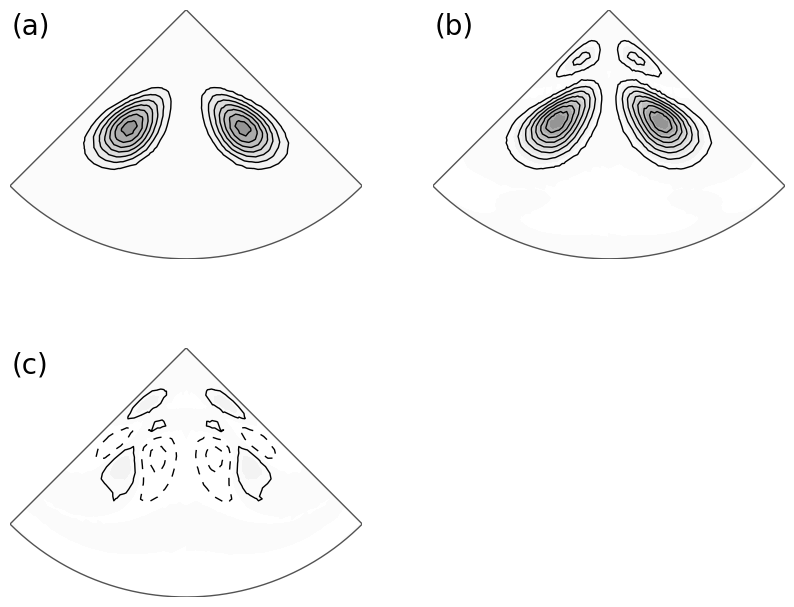
\includegraphics[width=0.9\linewidth]{OXgen.png}}
\caption{Распределение по сечению трубы $\Omega_x^2$ --- (a), вклад в производство $\Omega_x^2$ слагаемых, соответствующих выделенным в \eqref{OXgen_terms} --- (b), вклад остальных слагаемых в правой части \eqref{OX_eq} --- (с). Сплошные линии соответствуют положительным значениям, прерывистые --- отрицательным.}
\label{OXgen_pic}
\end{figure}

При анализе уравнения \eqref{OX_eq} обнаружено, что два слагаемых в правой части, а именно
\begin{equation}\label{OXgen_terms}
 - \overline{v'_x \frac{\d \omega'_x}{\d x}} + \overline{ \omega'_x \frac{\d v'_x}{\d x} },
\end{equation}
вносят определяющий вклад в производство средней продольной завихренности. Соответствующее сумме \eqref{OXgen_terms}  распределение в уравнении для $\Omega_x^2$ представлено на рис.~\ref{OXgen_pic}(b), а вклад остальных слагаемых правой части \eqref{OX_eq} показан на рис.~\ref{OXgen_pic}(c). Распределение генерации $\Omega_x^2$ выделенными в \eqref{OXgen_terms} членами практически совпадает по форме с распределением $\Omega_x^2$, тогда как вклад остальных членов не имеет выраженного распределения и более чем на порядок уступает по суммарному вкладу в генерацию $\Omega_x^2$. Таким образом, нет сомнения в том, что стационарные продольные вихри возникают в основном за счет действия выделенной в \eqref{OXgen_terms} пары слагаемых.

Отметим, что пульсации, соответствующие старшей собственной функции линейной задачи об устойчивости среднего стационарного течения, также демонстрируют приведенный выше механизм образования стационарных продольных вихрей. Важно, что это наблюдается только в том случае, когда при анализе устойчивости учитываются как продольная, так и поперечная составляющие среднего течения. Принято считать, что поперечное движение, определяя угловую неоднородность в распределении продольной скорости среднего течения, не может существенным образом влиять на свойства его устойчивости вследствие незначительности своей амплитуды. Поэтому при исследовании линейной устойчивости подобных течений, например, полосчатых структур в турбулентных потоках, наличие поперечного движения обычно не принимается во внимание. В нашем случае пренебрежение поперечным движением приводит к тому, что стационарное течение оказывается линейно устойчивым. Что еще более важно, наименее затухающее возмущение не воспроизводит при этом описанный механизм формирования продольных вихрей. Это связанно с тем, что форма пульсаций продольной завихренности $\omega'_x$ качественно меняется, хотя пульсации продольной скорости $v'_x$ сохраняют свою форму практически неизменной. Тем самым нарушается согласованность  $v'_x$ и $\omega'_x$, необходимая для обеспечения нужного вклада выражения \eqref{OXgen_terms} в производство продольной завихренности.

Каждое из двух слагаемых в \eqref{OXgen_terms} дает примерно половину общего вклада в производство средней продольной завихренности. Это значит, в частности, что колебания $\d v'_x/\d x$ и $\omega'_x$ положительно коррелированы в области концентрации положительной $\Omega_x$ и отрицательно коррелированы в области концентрации отрицательной $\Omega_x$. То же относится и к колебаниям $-v'_x$ и $\d \omega'_x/\d x$. Расчет соответствующих коэффициентов корреляции показывает, что они близки к $\pm1$ в соответствующих областях. 


\section{Механизм возникновения пульсаций продольной завихренности}

Для выявления механизма формирования такой связи между пульсациями продольных компонент скорости и завихренности рассмотрим уравнение эволюции $\omega'_x$, получающееся вычитанием \eqref{OX_eq} из \eqref{ox_eq}:
\begin{multline}\label{ox1_eq}
\pd{\omega'_x}{t} - \nu \nabla^2 \omega'_x = - (\V - \c, \nabla) \omega'_x - (\v', \nabla) \Omega_x
+(\Om, \nabla) v'_x + (\om', \nabla) V_x -\\- (\v', \nabla) \omega'_x  + (\om', \nabla) v'_x  + \overline{(\v', \nabla) \omega'_x)}  - \overline{(\om', \nabla)}
\end{multline}
Работать удобнее с уравнением, описывающим изменение среднего квадрата пульсаций продольной завихренности $\overline{\omega'^2_x}$, получающимся умножением на $2\omega'_x$ каждого из слагаемых в \eqref{ox1_eq} и последующим осреднением по времени. Как и раньше, осреднение по времени производится в подвижной системе отсчета. Слагаемые в этом уравнении не зависят от времени, сумма слагаемых в правой части балансируется вязким членом в левой части. Как и в предыдущем случае, среди всех слагаемых правой части удается выделить существенные, ответственные за возникновение пульсаций $\omega'_x$.


Распределение $\overline{\omega'^2_x}$ по сечению трубы с максимальным уровнем пульсаций изображено на рис.~\ref{ox1gen_pic}(a). Основные пульсации $\omega'_x$ наблюдаются в центре расчетной области около оси трубы. На месте расположения продольных вихрей также присутствуют пульсации $\omega'_x$, но меньшей интенсивности. В остальной части трубы их амплитуда близка к нулю. Обнаружено, что за генерацию пульсаций $\omega'_x$ в центральной части трубы и на месте продольных вихрей отвечают два разных механизма. Первый дает пульсации большей амплитуды, однако, за возникновение стационарных продольных вихрей ответственны пульсации, производимые вторым механизмом, так как именно они оказываются согласованными с пульсациями $v'_x$ нужным образом.


\begin{figure}[h]
\center{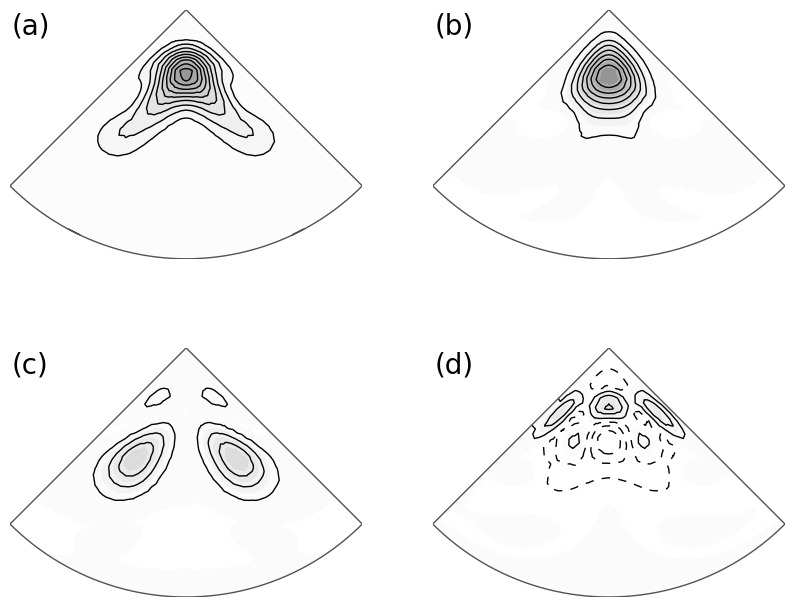
\includegraphics[width=0.9\linewidth]{ox1gen.png}}
\caption{Распределение среднего квадрата пульсаций продольной завихренности --- а, вклад в производство $\left<\omega'^2_x \right>$ слагаемых \eqref{ox1gen_add_terms} --- (b), слагаемого \eqref{ox1gen_main_terms} --- (c) и суммы остальных слагаемых правой части \eqref{ox1_eq} --- (d).}
\label{ox1gen_pic}
\end{figure}


Первый механизм формирования $\omega'_x$ связан с наличием нормальных к стенке вихрей в пульсационной составляющей движения. Можно провести аналогию между неустойчивостью, возникающей на полосе замедления, и неустойчивостью в следе за телом. Пульсационная составляющая движения напоминает дорожку Кармана. В ней можно выделить последовательность нормальных к стенке вихрей чередующегося знака, двигающихся вниз по полосе пониженной скорости. Им соответствуют области повышенной амплитуды пульсаций радиальной завихренности $\omega'_r$. Между полосой замедления и осью трубы имеется значительный радиальный градиент продольной скорости $\d V_x/ \d r$. В его присутствии нормальные к стенке вихри поворачиваются так, что приобретают продольную составляющую $\omega'_x$. Кроме того, наличие радиального градиента $\d V_x/ \d r$ связано с наличием угловой завихренности $\Omega_\theta = \d V_r / \d x - \d V_x / \d r$. Радиальная пульсационная завихренность $\omega'_r = \d v'_x / r \d \theta - \d v'_\theta / \d x$ за счет первого из слагаемых поворачивает стационарные угловые вихри так, что те также приобретают пульсационную продольную составляющую. В уравнении \eqref{ox1_eq} за описанный механизм отвечают слагаемые:
\begin{equation}\label{ox1gen_add_terms}
\frac{\d \omega'_x}{\d t} = \omega'_r \frac {\d V_x}{\d r} +
\frac{\Omega_\theta}{r} \frac{\d v'_x}{\d \theta} + ...
\end{equation}
Несмотря на то, что выделенные в \eqref{ox1gen_add_terms} слагаемые имеют противоположные знаки и в значительной степени компенсируют друг друга при сложении, их вклад в производство $\omega'_x$ значителен (см. рис.~\ref{ox1gen_pic}(b)). Они определяют форму пульсаций $\omega'_x$ в области между полосой замедления и осью трубы, где пульсации $\omega'_x$ достигают наибольшего значения. Эти пульсации, однако, практически не участвуют в образовании стационарной составляющей продольной завихренности. Это объясняется тем, что колебания $\omega'_x$, рождающиеся в результате описанного механизма, близки по фазе к колебаниям $v'_x$, так что сомножители каждого из слагаемых в выражении \eqref{OXgen_terms} оказываются в противофазе и при осреднении дают близкие к нулю значения.


Второй механизм образования пульсаций продольной завихренности $\omega'_x$ связан с перераспределением уже существующей стационарной продольной завихренности $\Omega_x$ за счет пульсационной составляющей продольной скорости $v'_x$ (эффект сжатия/растяжения вихревых линий). В уравнении \eqref{ox1_eq} за описываемый механизм отвечает слагаемое
\begin{equation}\label{ox1gen_main_terms}
\frac{\d \omega'_x}{\d t} = \Omega_x \frac {\d v'_x}{\d x} + ...
\end{equation}
Выделенное в \eqref{ox1gen_main_terms} слагаемое стремится произвести пульсации $\omega'_x$, пропорциональные $\d v'_x / \d x$, что обеспечивает наибольшую эффективность образования $\Omega_x$ посредством их нелинейного взаимодействия. Важно, что коэффициентом пропорциональности в \eqref{ox1gen_main_terms} выступает значение средней продольной завихренности, таким образом, механизм включается именно в областях концентрации $\Omega_x$. При этом производимые пульсации $\omega'_x$ положительно пропорциональны пульсациям  $\d v'_x / \d x$ при $\Omega_x>0$ и отрицательно пропорциональны при $\Omega_x<0$, что обеспечивает максимально возможную эффективность производства средней продольной завихренности нужного знака посредством второго из слагаемых выражения \eqref{OXgen_terms}. Очевидно, что пульсации $-v'_x$ и $\d \omega'_x / \d x$ в этом случае также согласованы нужным образом, так что первое слагаемое \eqref{OXgen_terms} близко по значению ко второму.


На рис.~\ref{ox1gen_pic}(c) приведен вклад выделенного в \eqref{ox1gen_main_terms} слагаемого в производство $\overline{\omega'^2_x}$. Нет сомнения, что именно это слагаемое определяет форму пульсаций в области существования продольных вихрей между полосами повышенной и пониженной скорости. Суммарный вклад других слагаемых правой части \eqref{ox1_eq}, не попавших на рис.~\ref{ox1gen_pic}(b,c), изображен на рис.~\ref{ox1gen_pic}(d). Эти слагаемые не имеют существенного значения в процессе генерации $\omega'_x$, их суммарный вклад не превышает нескольких процентов.

Описанный механизм генерации пульсаций продольной завихренности проявляется в области, где фазовая скорость волны, соответствующей пульсационной составляющей течения, близка по значению к локальной продольной скорости среднего течения. На удалении от точки генерации пульсаций, где фазовая скорость волны существенно отличается от средней скорости, выделенный в \eqref{ox1gen_main_terms} механизм генерации $\omega'_x$ практически не работает. Это объясняется тем, что в системе отсчета, связанной с волной, образующаяся посредством механизма \eqref{ox1gen_main_terms} $\omega'_x$ сносится вдоль трубы средним течением. При этом теряется согласованность фаз между $\d v'_x / \d x$ и $\omega'_x$, что делает её рост невозможным.


Описанный механизм генерации пульсаций продольной завихренности объясняет необходимость учета поперечного движения при исследовании устойчивости стационарного течения. Пренебрежение связанной с поперечным движением $\Omega_x$ делает невозможным генерацию $\omega'_x$ в форме, необходимой для сохранения поперечного движения, а следовательно и всего процесса самоподдержания пульсаций.

